\documentclass[12pt]{article}
\usepackage[utf8]{inputenc}
\usepackage{amsmath}
\usepackage{amssymb}
\usepackage{multicol}
\usepackage{fullpage}
\usepackage{bera}
\usepackage{xcolor}
\usepackage{hyperref}
\usepackage{graphicx}

\setlength{\parindent}{0pt}

\begin{document}

\begin{flushleft}
{\footnotesize Pontificia Universidad Católica de Chile\\
Departamento de Ciencia de la Computación\\
Computación: Ciencia y Tecnología del Mundo Digital\\
}
\begin{center}
{\huge\bf Tarea Chica 3: Máquinas de Turing}\\ \vspace{0.5cm}
Profesor Denis Parra \\
Manuel Espinoza Quintero \\

\rule{\linewidth}{0.1mm}
\end{center}
\end{flushleft}

La tarea es escribir una máquina de Turing M que acepte lo siguiente:

$$L=\{d\# n_1\# n_2 \# n_3 \#...\# n_k | \; \textrm{con} \; n_i-n_{i+1}=d\}$$

Por lo tanto, un ejemplo de input sería:

$$00011\#10100\#10001\#01110\#01011$$

La forma en que se escribe el código de la maquina es:

\begin{equation*}
    \begin{split}
        & \mathtt{{\scriptstyle [1]} \quad estado_a, n_1, n_2, ..., n_k}\\
        & \mathtt{{\scriptstyle [2]} \quad estado_b, n'_1, n'_2, ..., n'_k, mov_1, mov_2, ..., mov_k}
    \end{split}
\end{equation*}

Donde $\mathtt{estado_a}$ es el estado actual de la maquina, $\mathtt{n_1, n_2, ...,n_k}$ son los valores que hay en las $k$ cintas, en ese orden. La segunda linea se lee si se cumple la primera, y cambia de estado al $\mathtt{estado_b}$ y los valores en las cintas cambian a $\mathtt{n'_1, n'_2, ...,n'_k}$. Por último, $\mathtt{mov_1, mov_2, ..., mov_k}$ son los movimientos de las cintas los cuales pueden ser: $\mathtt{<, >, -}$, izquierda, derecha y mantenerse, respectivamente.\\

\textbf{Lógica:}\\
La lógica utilizada es principalmente restar d al número del input y verificar con el que le sigue, y repetir el proceso hasta acabar con la sucesión. Los pasos que se realizan son descritos en el funcionamiento.

\textbf{Conceptos:}\\

$Q$: Conjunto finito de estados de la maquina para llegar al output.\\
$q_0$: estado inicial de la operacion, en este caso qcopy.\\
$\Gamma$:es el alfabeto de la máquina en este caso binario\\
$Q$: $\subseteq Q$ y se refiere a los estados finales. En este caso qAccept

\newpage
\textbf{Funcionamiento:}\\

\begin{enumerate}
\item \textbf{Qcopy:}

Al inicio se establece el estado inicial \textit{“qcopyd”} y el estado final \textit{“qAccept”}. Luego, se inicia copiando el primer numero binario del input (\textit{“d”}) en la segunda cinta. Esto con el objetivo de restar el \textit{“d”} a cada número de la primera cinta. Si en la primera cinta hay un 0, el estado se encarga de eliminarlo y escribir un 0 en la segunda, y lo mismo con el 1. Cada vez que copia un número las dos primeras cintas avanzan un espacio a la izquierda. Al encontrar el primer \# cambia de estado, ya que termino de copiar y se pasa al estado \textit{“volver”}.\par

\begin{figure}[h]
    \centering
    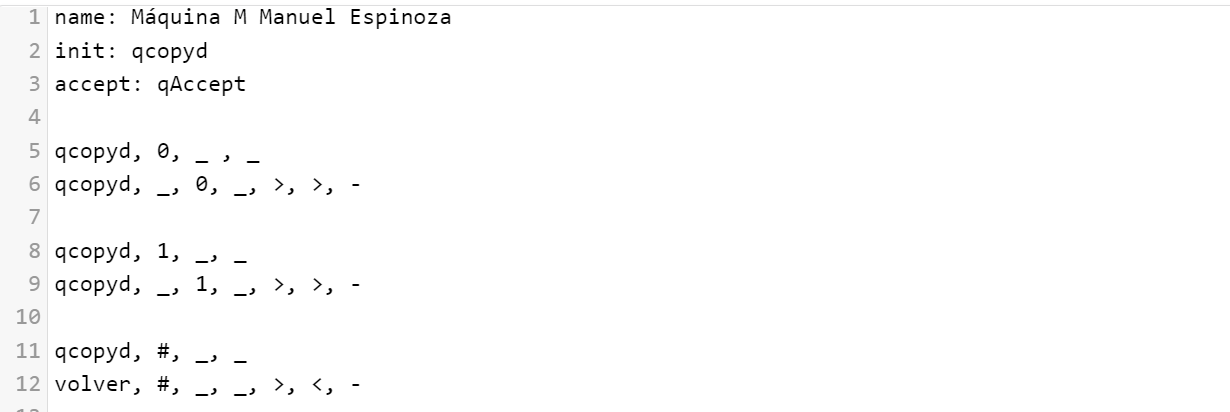
\includegraphics[width=\textwidth]{fotos/Screenshot 2021-11-26 173352.png}
    \caption{Inicio codigo y copia de "d"}
\end{figure}

\newpage
\item \textbf{Volver:}\\

Para restar \textit{“d"} de los números, es necesario equiparar las dos primeras cintas al igual que cuando hacemos una resta a mano. El estado volver simplemente copia lo mismo que encuentra en las dos primeras cintas y va retrocediendo la primera, hasta que encuentra el \# y ahí retrocede una casilla, siempre sin cambiar el valor de \textit{“d"}. Con los números ya nivelados se procede a realizar la resta, para lo cual se definió un estado \textit{“resta"}.


\begin{figure}[h]
    \centering
    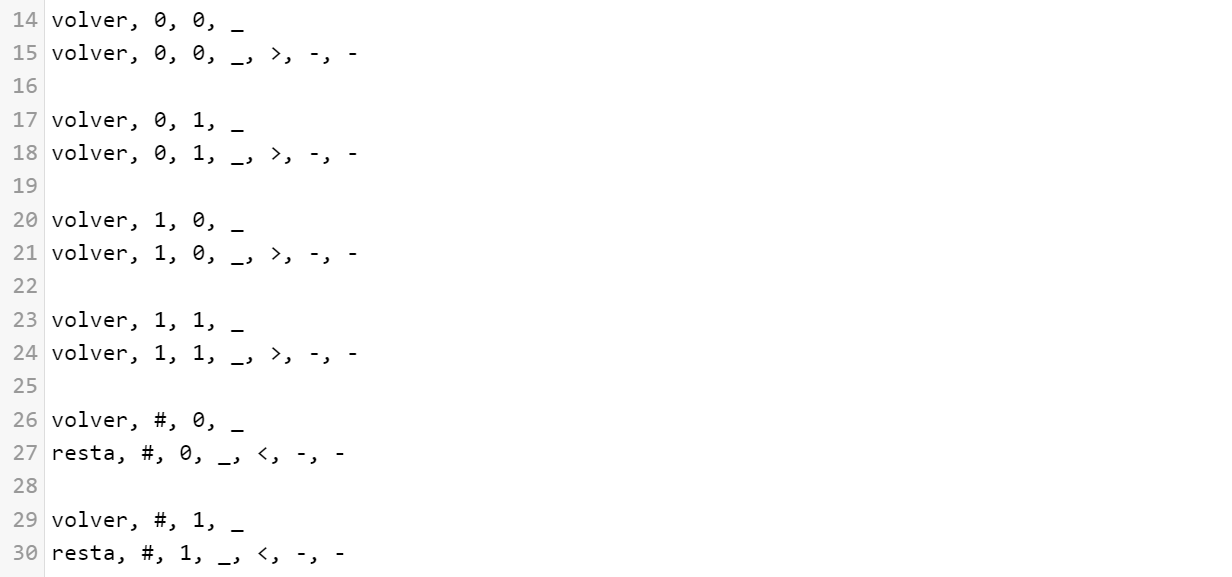
\includegraphics[width=\textwidth]{fotos/Screenshot 2021-11-26 175821.png}
    \caption{Retroceso de primera cinta}
\end{figure}


\newpage
\item \textbf{Resta:}\\
Para la resta de números binarios se puede asegurar que las siguientes combinaciones siempre son iguales:

\begin{itemize}
    \item $\mathtt{0} - \mathtt{0} = \mathtt{0}$
    \item $\mathtt{1} - \mathtt{1} = \mathtt{0}$
    \item $\mathtt{1} - \mathtt{0} = \mathtt{1}$
\end{itemize}

En cambio, cuando se tiene el caso $\mathtt{0} - \mathtt{1}$ se le pide una unidad prestada al número del lado izquierdo.Para ese caso, se definido un estado llamado \textit{"resta1"}, que tiene en consideración esa unidad prestada.\\

El proceso que realiza la maquina es leer las dos primeras cintas y ver a que caso corresponde, y escribir el resultado en la tercera cinta, y las mueve todas una posición a la izquierda.

\begin{figure}[h]
    \centering
    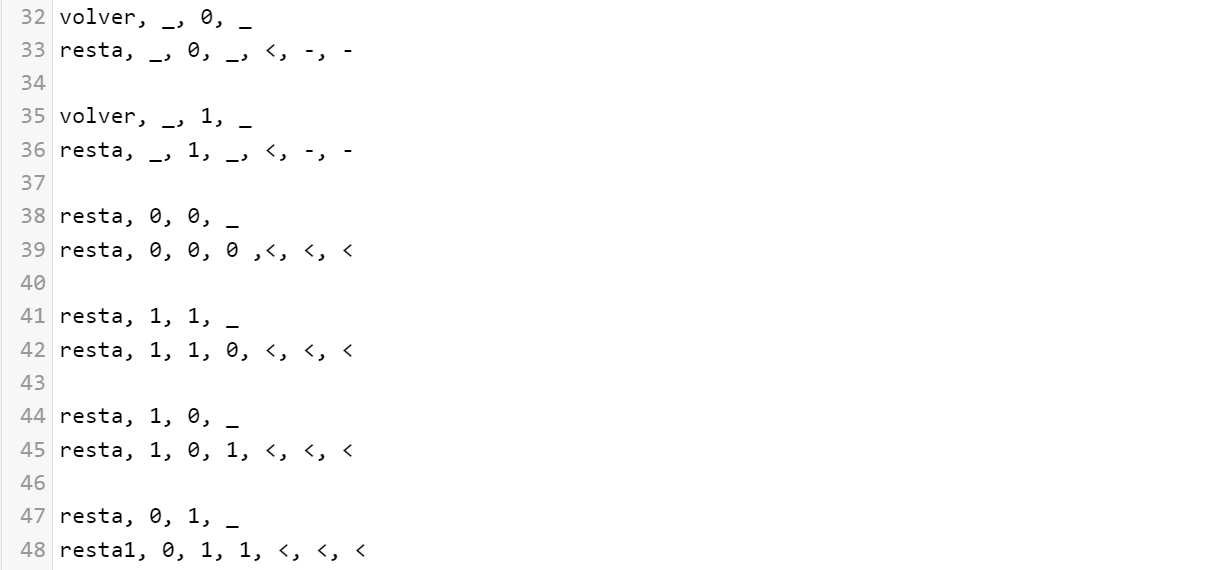
\includegraphics[width=\textwidth]{fotos/Screenshot 2021-11-27 181308}
    \caption{Proceso de resta}
\end{figure}

\newpage

\item \textbf{Resta1:}\\
Cuando la maquina entra en el estado \textit{resta1}, las combinaciones se dan diferentes, si se tiene 1-1, eventualmente va a volver a tener que pedir prestado, por lo tanto, el resultado es 0 y se sigue en el estado resta1. Si el caso es 0-1 o 0-0, no se le puede pedir prestado, y se sigue con el siguiente a la izquierda. En estos casos, los resultados van a ser 0 y 1 respectivamente, ya que al número que le restamos le va a llegar un 1 prestado y 1-1=0, 1-0=1. Por último, el caso que se tenga 1-0 en la columna de la cual se le pide prestado, se asume que el resultado va a ser 0, ya que el 1 se va prestado a la anterior operación, y en este caso se vuelve al estado \textit{resta}. Al encontrar el /# se entiende que se termino de restar d al número, por lo que vuelve al estado volver, que se encarga de mover la primera cinta para comparar el siguiente numero de la cinta con el resultado obtenido.

\begin{figure}[h]
    \centering
    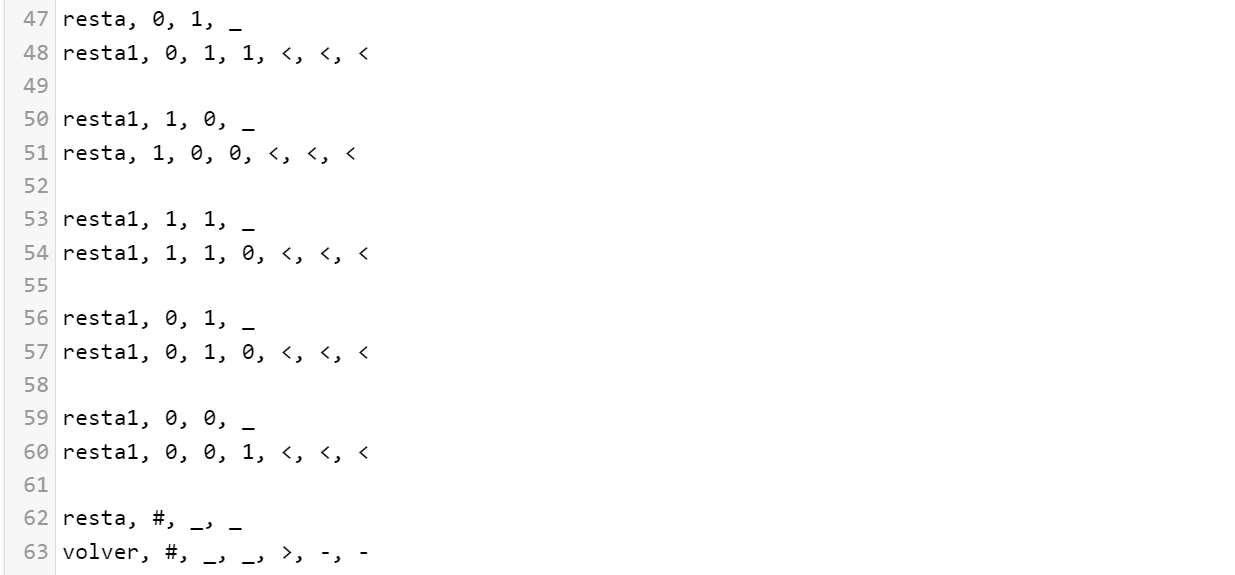
\includegraphics[width=\textwidth]{fotos/Screenshot 2021-11-27 181502}
    \caption{Proceso de resta}
\end{figure}

\newpage
\item \textbf{Volver y comparar:}\\

El proceso de comparación revisa que tanto en la primera como tercera cinta sea el mismo número, un 0 o un 1, si ese es el caso, pasa al siguiente. Si no coinciden quiere decir que el input es rechazado y la maquina se cae.

\begin{figure}[h]
    \centering
    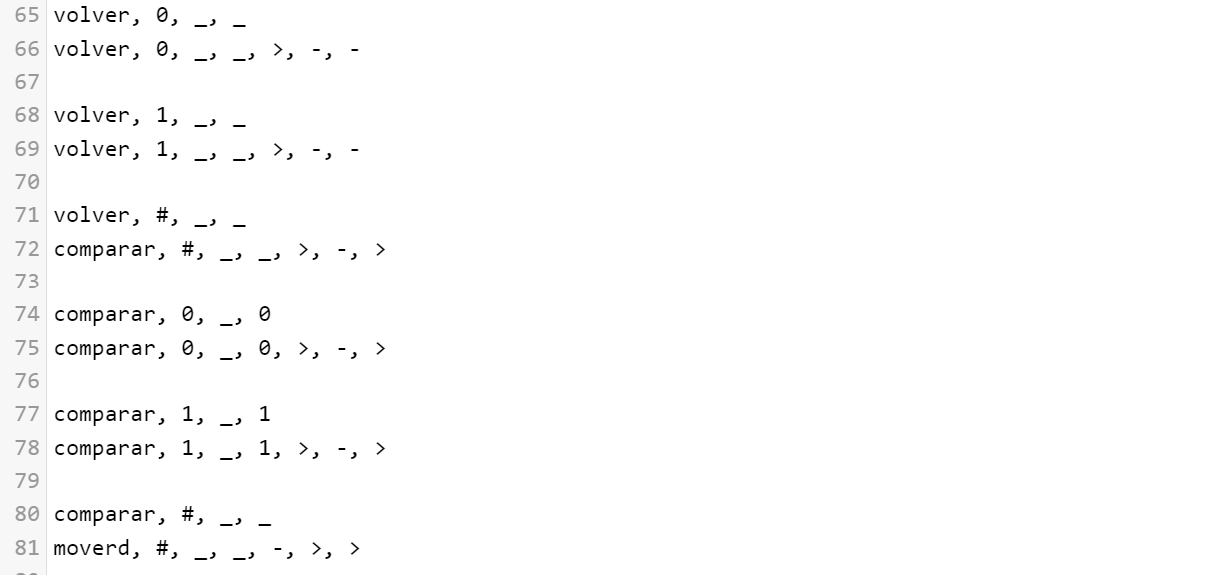
\includegraphics[width=\textwidth]{fotos/Screenshot 2021-11-27 181838}
    \caption{Retroceso primera cinta y comparación de valores}
\end{figure}


\newpage
\item \textbf{Moverd y qAccept:}\\

Para finalizar se mueve la segunda y tercera cinta para equipararlas y volver a realizar el proceso de resta con el siguiente número. Si se cumple que todas las cintas están vacías, significa que finalizaron los números a verificar y se pasa al estado qAccept.

\begin{figure}[h]
    \centering
    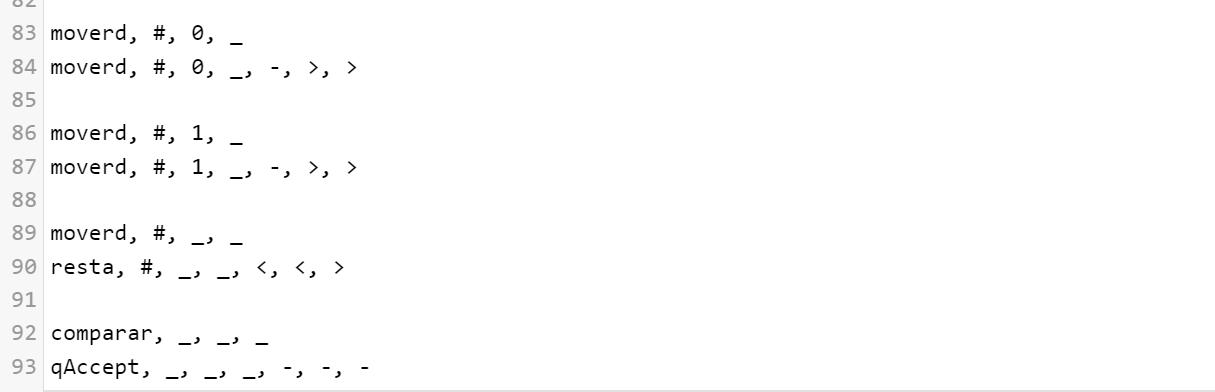
\includegraphics[width=\textwidth]{fotos/Screenshot 2021-11-27 182052}
    \caption{Avance de cintas 2 y 3 y estado final}
\end{figure}

\end{enumerate}
\end{document}
